\chapter{Proof of xyz}
\label{appendix}
\thispagestyle{myheadings}

\graphicspath{{Appendix/Figures/}}

\section{Memory and Process in Operation Systems}
\label{sec:history}
A process is a section of computation job. A process can work on a CPU core. We can devide process as well.
Basically, each process does not share thier memory. However, for multiprocessing, we could avoid this restriction.
Processes can be represented as tree structure, because a process may create onther child processes.
Process has 4 states, new, running, waiting, and ready. 
Process is represented in process control block (PCB) with state type, process ID, registers, and so on.
The scheduling for process assigning to CPU core is implemented in queues containing PCB. There are two main queues in this scheduler: 
ready queue and wait queue. The head of process in ready queue is selected for execution and once the process requested I/O request or 
production of child process, the running process will be stored n wait queue. Once the request that the process waiting for end, 
the waiting process will be pushed tail of ready queue. 

Processes executing concurrently in the operating system may be either independent processes or cooperating processes excuting in the system.
A process is indepenedent if it does not share data with any other processes. A process cooperating if ti can affect or be affected by the 
other processed executing in the system. In cooperating process, there are two kinds, shared memory and message passing. 
In shared memory, it removes restriction of not interfering memory region. Message passing can be useful for destribution systems as well.

For a pair of processes to communicate throught message, a socket is needed to be established. 
A socket is identified by an IP address concatenated with a port number. When two process communicate, each process will have socket. 
If another process of the same machine wants to communicate, we need new socket to be established. The protocol used in the socket connection
can be TPC and UDP.

\section{Miltithreading and Parallelism}
\label{sec:history}
A thread is a basic unit of CPU usilization, so that a process can have multiple thread. Threads shares mainly code and data. 
Multithreaing is increasingly popular as the multicore programming becomes in common, becasue we can run multiple thread on different core.
Creating thread is much cheaper than creating process and it shares resources so that we do not need addtional methods to allow threads to 
communicate each other, such as sharing memory and message passing.

\section{Memory management in Operation System}
\label{sec:history}
In computer storage hierarchy, the closest strage to CPU is register. It is built into each CPU core and accessible within one cycle of the CPU clock.
However, the same cannot be said of main memory, which is accessed via a transaction on the memory bus. This takes many cycles of the CPU clock.
The remedy is to add fast memeory between the CPU and main memory, typically on the CPU chip for faster access. Such a cache plays a role for this.

For the layout of main memory, it must be ensured that each process has a separate memory space, including operation system. 
The base register and limit register, whose roles are lower boound of memory region and specific size of range respectively, can achieve that goal. 

Usually a program resides on a disk as binary excutable file. To run, the program must be brought into memory and placed within the context of a crocess.
The process is binded to corresponding parts of the physical memory. Binding program to memeory address is staging process. 
There three stages: compile time, load time excution time. The source program is compiled by compiler producing object file. 
After the compilation, the object file is linked with other object file by linker creating executable file . 
Finally, the executable file will be loaded to run execute. At this run time dynamic linbrary link can be done.

If where the process will reside in memory at compile time, absolute code is generated. If this is unknown at the time, 
the binding will be done at load time. At this time, the compiler must generate relocatable code. Otherwise, the binding will be done at 
execution time.

A process does not interact with addresses of physical memory, instead virtual memory. The memory-management unit (MMU) takes roles to map 
logical address to physical address. OS needs to ensure that any of physical memory spaces of processes do not overlap. 
Since one process can be created and deleted and the corresponding memory space should be de/allocated, 
optimization for use of physical memory space is important; we need to allocate memory contiguously avoiding fragmentation.

There are several approaches to deal with this problems. However, we will focus on paging here, which is the most used method OS use to manage memory.
A frame and page are a unit of Separated physical and virtaual memory space in fixed size (4KB or 8KB) respectively.
A process can use as many as pages and correspinding frames obtained by page table matching. This strategy does improve external fragmentation, but not for internal fragmentation.
The smaller size of page has smaller fragmentation, but mapping from page to grame has overhead and also disk I/O is more efficient when the amount of data transfered is larger.



\section{Demand Paging}
\label{sec:history}
A process can have mutiple pages. However, loading entire executable code from sendory storage to memory is not necessarily needed to 
get jobs done. A storategy used in several operating systems is loading only the portion of programs that are needed, demand page. 

In the storatege, some pages currently used are in memory and the others are in secondary storage. 
The page table specifies whether pages are valid or invalid, which means are in memory or not. 
Access to a page marked invalid causes page fault and some steps to resolve the error will be required. 

The first part of process of demand pageing would be that we check an internal table to check whether the reference is valide or invalid.
If the reference is valid, the process reads the content from the memory. Otherwise, we terminates the process and find the free frame in 
physical memory. Then, we schedule a secondary storage operation to read the desired page into newly allocated frame. 
When the storage complete reading the page, we modify the internal table to indicate the page is now in memory. 
Finally, we restart the instruction that was interrupted. 

However, there would be a case where the memory does not have any free frame. In this case, a victim frame that will be replaced with new comming frame should be selected. 
To perform this selection efficiently, a modify bit is tracked for each frame or page. The modify bit represents whether the page is modified since it is loaded from secondary storage. 
If the page or frame is modified, when we swap page we need to update the content in the secondary storage. However, it is not modified, we can simplly delete the frame and replace with new frame.



\section{Copy on Page}
\label{sec:history}
When a parent process creates child process and if these process shares contents on particular page and modify it, 
only the page which has the contenst will be copied.


\section{Threads and Concurrency}
\label{sec:history}

\section{BLAS LAPACK}
\label{sec:history}

Basic Linear Algebra Subprograms (BLAS) are standard building blocks for basic vector and matrix operations. There are 3 levels of operation. The level 1 BLAS performs scalar, 
vector and vector-vector operations, the level 2 BLAS performs matrix-vector operation, and the level 3 BLAS performs matrix-matrix operation. 

LAPACK is developed on BLAS and has advanced functionalities such as LU decomposition and Singular Value Decomposition (SVD). Dense and banded matrices are handled, but not general 
sparse matrices. The initial motivation of development of LAPACK was to make the widely used EISPACK and LINPACK libraries run efficiently on shared-memory vector and parallel processors. 
LINPACK and EISPACK are inefficient because their memory access patterns disregard the multi-layered memory hierarchies of the machines, thereby spending too much time moving data. 
LAPACK addresses this problem by recognizing the algorithms to use block matrix operations, such as matrix multiplication, in the innermost loops. These block operations can be optimized for each architecture to account for the memory hierarchy, 
and so provide a portable way to achieve high efficiency on diverse modern machines. However, LAPACK requires that highly optimized block matrix operations be already implemented on each machine. 

ARPACK is also a collection of linear algebra subroutines which is designed to compute a few eigenvalues and corresponding eigenvectors from large scale matrix. 
ARPACK is based upon an algorithmic variant of the Arnoldi process called the Implicitly Restarted Arnoldi Method (IRAM). 
When the matrix is symmetric it reduces to a variant of the Lanczos process called the Implicitly Restarted Lanczos Method(IRLM). The Arnoldi process only interacts with the matrix via matrix-vector multiplies. 
Therefore, this method can be applied to distributed matrix operations required in big data analysis.


The original BLAS and LAPACK are written in Fortran90. Linear algebra library used for Spark is netlib-java, which is a Java wrapper library for Netlib, C API of BLAS and LAPACK. 
The reason why the developers addressed to use this package is that the BLAS and LAPACK are already bug free and implementing linear algebra library from scratch can usually buggy. 

However, the main advantage of use of BLAS and LAPACK is system optimized implementation. So if we implement original Fortran linear algebra library, it cannot perform as well as BLAS and LAPACK. 
And the performance would not be such different from one of implementation in Java or Rust.  If we want to test only memory management between Rust and Java, 
it can be enough implementation of linear algebra operation from  pure Java and Rust sacrificing the best performance taking advantage of system optimization. 


\section{Netlib-Java}
\label{sec:history}

Netlib-java is a Java wrapper of BLAS, LAPACK, and ARPACK. Netlib-java choose  implementation of linear algebra depending on installation of the libraries. 
First, if we have installed machine optimised system libraries, such as Intel MKL and OpenBLAS, netlib-java will use these as the implementation to use. 
Next, it try to load netlib references which netlib-java use CBLAS and LAPCKE interface to perform BLAS and LAPACK native call. 
The last option is to use f2j which is intended to translate the BLAS and LAPACK libraries from their Fortran77 reference source code to Java class files, 
instead of calling native libraries by using Java Native Interface (JNI). 

We can use JNI to call native libraries from Java. The JNI is a native programming interface which allows Java code that runs inside a Java Virtual Machine (VM) 
to interoperate with applications and libraries written in other programming languages. 

\section{Create Java interface of CBLAS with JNI}
\label{sec:history}
\begin{enumerate}
    \item Download BLAS and build using make file. In the figure2.1, the built file is libblas.a and the header file is blas.h.
    \item Download CBLAS and build using make file (I am not sure whether we should build archive file or shared library). In figure, the build file would be libcblas.a or libcblas.dylib and header file is cblas.h.
    \item Create java file which will be the Java interface of CBLAS.
    \item Compile java file with -h header flag to create class file (CBLASJ.class) and header file (CBLASJ.h).
\begin{lstlisting}[language=bash]
    $ javac -h . CBLASJ.java
\end{lstlisting}
    \item Create C file (CBLASJ.c) which will bind Java interface and CBLAS library. And compile it with JNI to create object file (CBLASJ.o).
\begin{lstlisting}[language=bash]
    $ gcc -c-fPIC -I${JAVA_HOME}/include -I${JAVA_HOME}/include/darwin CBLASJ.c
\end{lstlisting}
    \item Compile shared library linking library (libcblas.a or libcblas.dylib) object file (CBLASJ.o).
\begin{lstlisting}[language=bash]
    $ gcc -o libcblas.dylib (or libcblas.a) CBLASJ.o 
\end{lstlisting}
\end{enumerate}

\begin{figure}[htb]
    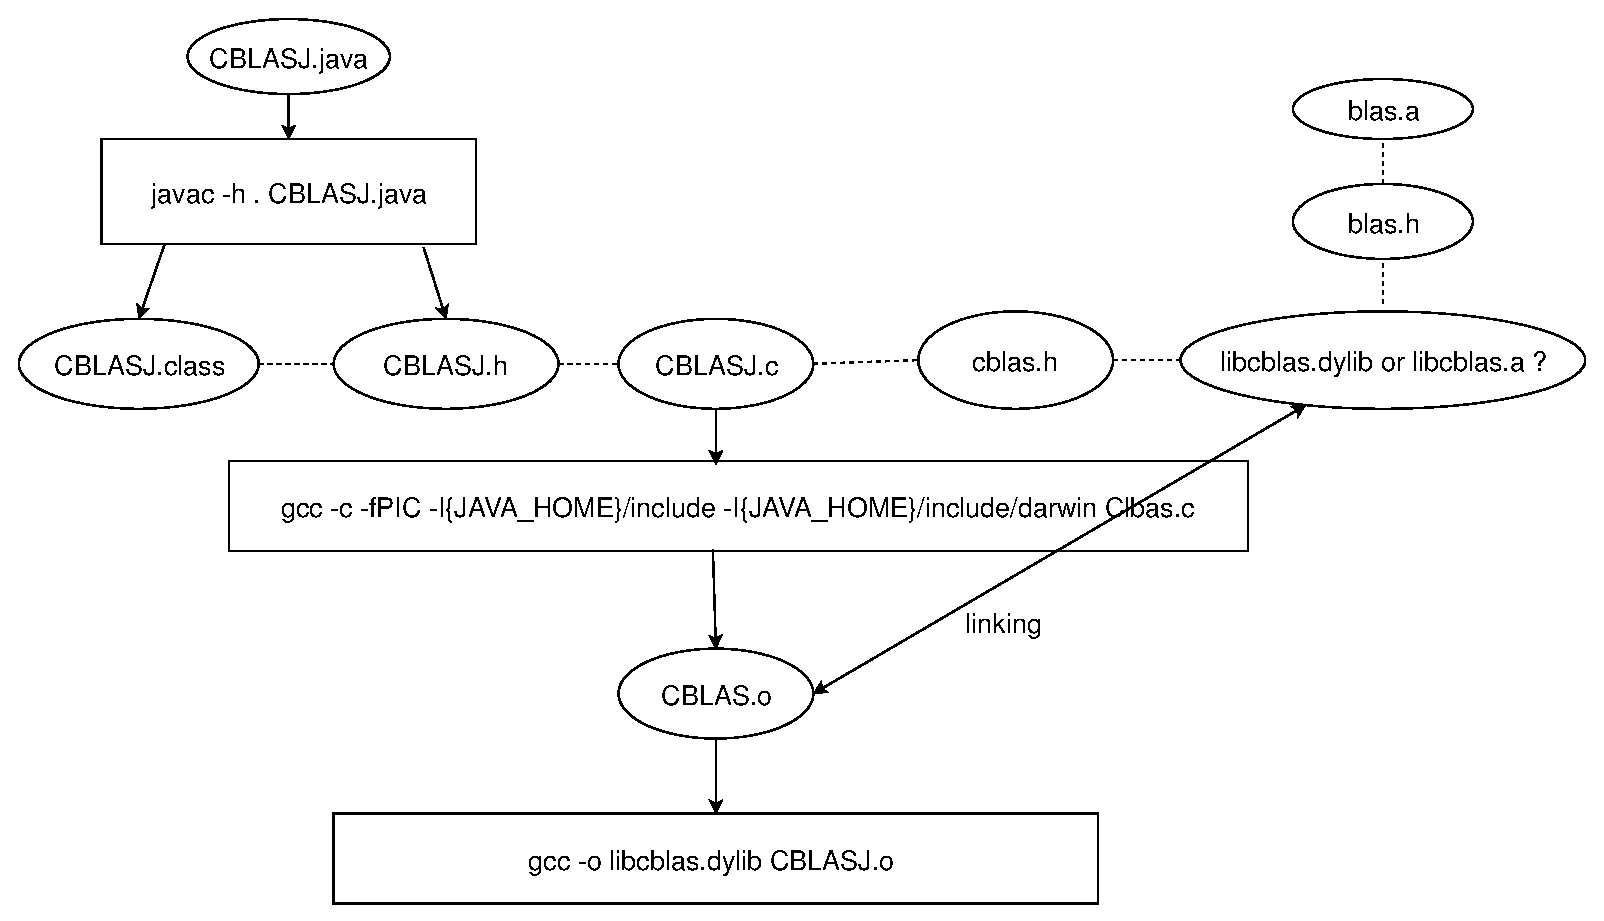
\includegraphics[width=15cm]{cblas_with_jni.eps}
    \caption{Integration of Native Methods }
    \label{fig:Sampling}
\end{figure}



\section{Matrix Computation and Optimization in Apache Spark}
\label{sec:history}

Matrix operation is a fundamental part of machine learning. Apache Spark provides implementation for distributed and local matrix operation. 
To translate single-node algorithms to run on a distributed cluster, Spark addresses separating matrix operations from vector operations and run matrix operations on the cluster, 
while keeping vector operations local to the driver. 

Spark changes its behavior for matrix operations depending on the type of operations and shape of matrices. For example, Singular Value Decomposition (SVD) for a square matrix is performed in distributed cluster, 
but SVD for a tall and skinny matrix is on a driver node. This is because the matrix derived among the computation of SVD for tall and skinny matrix is usually small so that it can fit to single node.

Spark uses ARPACK to solve square SVD. ARPACK is a collection of Fortran77 designed to solve eigenvalue problems. ARPACK is based upon an algorithmic variant of the Arnoldi process called the Implicitly Restarted Arnoldi Method (IRAM). 
When the matrix A is symmetric it reduces to a variant of the Lanczos process called the Implicitly Restarted Lanczos Method (IRLM). 
ARPACK calculate matrix multiplication by performing matrix-vector multiplication. So we can distribute matrix-vector multiplies, and exploit the computational resources available in the entire cluster. 
The other method to distribute matrix operations is Spark TFOCS. Spark TFOCS supports several optimization methods.

To allow full use of hardware-specific linear algebraic operations on single node, Spark uses the BLAS (Basic Linear Algebra Systems) interface with relevant libraries for CPU and GPU acceleration. 
Native libraries can be used in Scala are ones with C BLAS interface or wrapper and called through the Java native interface implemented in Netlib-java library and wrapped by the Scala library called Breeze. 
Following is some of the implementation of BLAS.

\begin{itemize}
    \item f2jblas -  Java implementation of Fortran BLAS
    \item OpenBLAS - open source CPU-optimized C implementation of BLAS
    \item MKL - CPU-optimized C and Fortran implementation of BLAS by Intel
\end{itemize}

These have different implementation and they perform differently for the type of operation and matrices shape. 
In Sark, OpenBlas is the default method of choice. BLAS interface is made specifically for dense linear algebra. 
Then, there are few libraries that efficiently handle sparse matrix operations.

\section{Memory Management of each Linear Algebra Library}
\label{sec:history}

The pure Java linear algebra library, such as La4j, EJML, and Apache Common Math, 
use normal GC performed by JVM to manage memory. This is because the implementation of these libraries are in purely Java.

Netlib-java, Jblas or other simple Java wrapper of BLAS, LAPACK, and ARPACK with Java Native Interface (JNI) use normal GC as well. 
This is because the native code deals with Java array by obtaining a reference to it. After the operation, 
the native method releases the reference to the Java array with or without returning new Java array or Java primitive type object. 

ND4J has two types of  its own memory management methods, GC to pointer of off-heap NDArray, and MemoryWorkspaces. 
ND4J used off-heap memory to store NDArrats, to provide better performance while working with NDArrays from vative code such as BLAS and CUDA libraries. 
Off-heap means that the memory is allocated outside of the Java heap so that it is not managed by the JVM’s GC. NDArray itself is not tracked by JVM, 
but its pointer is. The Java heap stores pointer to NDArray on off-heap. When a pointer is dereferenced, this pointer can be a target of JVM’s GC and when it is collected, 
the corresponding NDArray will be deallocated. When using MemoryWorkspaces, NDArray lives only within specific workspace scope. 
When NDArray leaves the workspace scope, the memory is deallocated unless explicitly calling method to copy the NDArray out of the scope.
